\subsection{公司破产预测}
\subsubsection{模型建立}
\paragraph{高斯判别分析}
基于数据分布检验,互信息选择的单个变量服从高斯分布,从而变量的组合服从
多维正态分布。这正符合高斯判别分析(Gaussian Discriminant Analysis, GDA)
对于特征数据分布的要求。在GDA中,需要进一步假设
二元取值的数据标签(破产与否)服从伯努利分布。
将数据集记为$\{(x^{(i)}, y^{(i)})\}_{i=1}^m$,从而上述分布
定量表达为:
\begin{align}
    \begin{split}
    y &\sim \text{Bernoulli} (\phi) \\
    x|y = 0 &\sim \mathcal{N}(\mu_0, \Sigma) \\
    x|y = 1 &\sim \mathcal{N}(\mu_1, \Sigma)
    \end{split}
    \label{eq:assumptions-mul-gaussian}
\end{align}
这里为了简化模型,认为$x|y = 0$和$x|y = 1$的协方差矩阵相同。
利用最大似然估计寻求参数$\mu_0, \mu_1, \Sigma, \phi$,
为此最大化联合似然函数:
\begin{equation*}
    \mathcal{L}(\mu_0, \mu_1, \Sigma, \phi)=\Pi_{i=1}^{m}
p(x^{(i)}, y^{(i)}; \mu_0, \mu_1, \Sigma, \phi)
\end{equation*}
进一步最大化对数似然函数:
\begin{align}
\begin{split}
    \ell (\mu_0, \mu_1, \Sigma, \phi) &=\log \mathcal{L}(\mu_0, \mu_1, \Sigma, \phi) \\
    &=\sum\limits_{i=1}^{m} \log p(x^{(i)} | y^{(i)}) + \log p(y^{(i)})
\end{split}
    \label{eq:log-likelihood}
\end{align}
式\ref{eq:log-likelihood}中分别使参数的梯度为零,求解得到:
\begin{align}
    \begin{split}
    \phi &= \frac{1}{m}\sum\limits_{i=1}^{m} \mathbf{1}\{y^{(i)}=1\} \\
    \mu_j &= \frac{\sum_{i=1}^{m}\mathbf{1}\{y^{(i)}=j\}x^{(i)}}{
        \sum_{i=1}^{m}\mathbf{1}\{y^{(i)}=j\}
    } \\
    \Sigma &= \frac{1}{m}\sum\limits_{i=1}^{m}(x^{(i)}-\mu_{y^{(i)}})
    (x^{(i)}-\mu_{y^{(i)}})^T
    \end{split}
    \label{eq:MLE-GDA}
\end{align}
其中$\mathbf{1}\{\cdot\}$是示性函数。利用式\ref{eq:MLE-GDA}求解参数的最大似然估计,
在预测阶段,模型输出:
\begin{equation*}
    \arg \max_{y} p(y|x) = \arg \max_{y} p(y)p(x|y)
\end{equation*}
\par 值得一提的是,如果将$p(y=1|x; \mu_0, \mu_1, \Sigma, \phi)$表示为
$x$的函数,可以得到
\begin{equation*}
p(y=1|x; \mu_0, \mu_1, \Sigma, \phi)=\frac{1}{1+\exp (-\theta^T x)}
\end{equation*}
其中$\theta$是参数$\mu_0, \mu_1, \Sigma, \phi$的函数。这正是逻辑回归的
表达式,说明在正态分布的假设下,高斯判别分析的输出结果与逻辑回归形式一致
\footnote{
    虽然边界函数形式一致,但是两者形成的边界有差别
}。但是高斯判别分析利用了假设\ref{eq:assumptions-mul-gaussian},
对数据的分布有更强的要求,在数据量较少、数据真实分布与假设一致的情况下,
高斯判别分析的分类效果往往好于单纯的逻辑回归。

\paragraph{随机森林}
决策树选择一个轴(对应一个特征)和相应的阈值,对于高维空间进行划分,
这样的思路对于而二分类问题有较好的效果。
但是一个利用所有特征形成的决策树通常偏差较小、方差较大,这是由决策树的分割特点
决定的。如果考虑$n$个相同模型,各自的误差为随机变量$X_i$,并进一步假设
$Var(X_i)=\sigma^2,Cov(X_i,X_j)=\rho\sigma^2$,
则误差均值的方差为
\begin{align*}
    \begin{split}
        Var(\bar{X})&=\frac{1}{n^2}\sum\limits_{i,j}Cov(X_i, X_j) \\
        & = \rho\sigma^2 + \frac{1-\rho}{n}\sigma^2
    \end{split}
\end{align*}
增加模型的数量可以使得第二项减小,但是会显著增加计算成本。利用统计的方法
可以使$\rho$减小,例如\textit{Bootstrap}方法。如果在形成单个决策树时
使用不同的特征集合,可以进一步减少模型之间的相似度,从而减小方差。
但是由于单个决策树没有关于所有特征的信息,所以不可避免的模型的偏差会增加。
\par 使用Gini指数$Gini(x)=1-\sum_{i=1}^n (p_i)^2$(本问题中$n=2$)
作为损失函数,通过数值方法进行求解,确定每一次用于分割的特征。
假设总特征数量为$p$,在随机森林中,每个决策树使用$[\sqrt{p}]$个特征,
同时样本利用\textit{Bootstrap}方法从总样本集中取出。
\par 随机森林的特征处理分为以下几步:
\begin{enumerate}
    \item 检查并替换异常值。计算一列数据的下四分位数(记为$Q_1$)和
    上四分位数(记为$Q_3$),进而得到四分位距(Interquartile Range, IQR)
    $\coloneqq Q_3-Q_1$。在$[Q_1-1.5IQR, Q_3+1.5IQR]$之外的数据认为是
    异常值,将其相应替换为上下限值。其中1.5是一个经验值,可以人为规定。
    第一步的过程展示在图\ref{fig:IQR-outlier-detection}中。
    \begin{figure}[h]
        \centering
        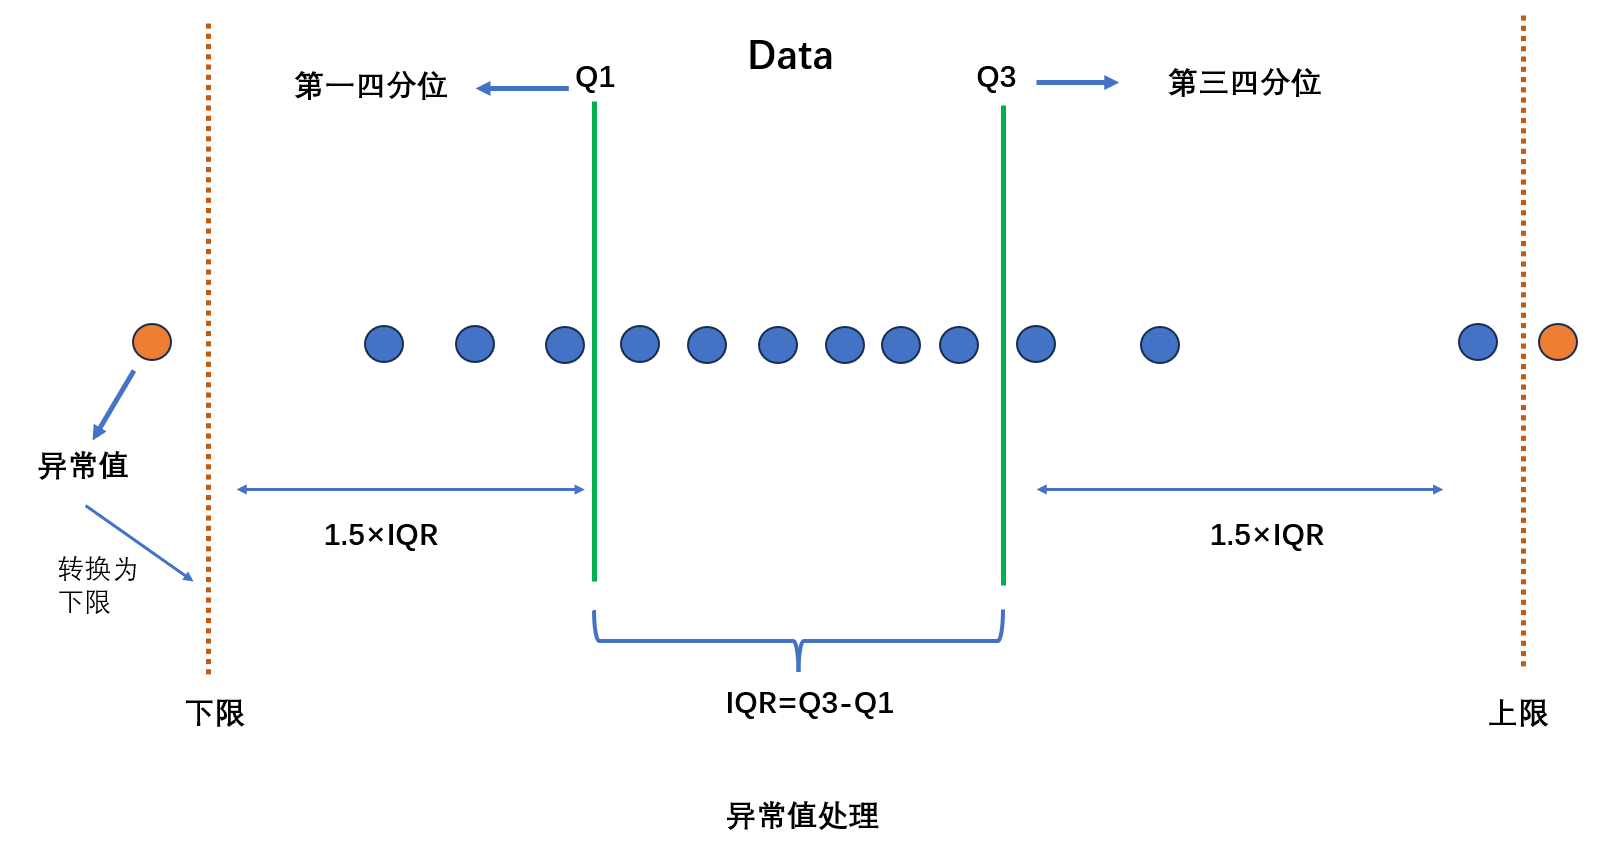
\includegraphics[width=.6\textwidth]{images/IQR_outlier_selection.png}
        \caption{IQR方法检测并替换异常值过程}
        \label{fig:IQR-outlier-detection}
    \end{figure}
    \item 去除冗余特征。分为两部分:
    \begin{enumerate}
        \item 删除方差小于0.1的特征,即变动幅度非常小的特征
        \item 对于协方差大于0.8的特征组,保留其中一个
    \end{enumerate}
    \item 过采样平衡数据集。观察到数据集中存在不平衡问题,先将原始数据
    按照0.2的测试集比例进行划分,对于划分得到的训练集,
    利用\textit{BorderlineSMOTE}过采样方法处理,平衡其中的正负样本
    数量。传统的\textit{SMOTE}方法主要分为四个步骤:
    \begin{enumerate}
        \item 从少数类样本中随机选择一个样本
        \item 使用一种范数找到该样本的$k$个最近邻样本(取$k=5$)
        \item 从这$k$个近邻样本中随机选择一个样本,
        在选择的样本和原始样本之间插值生成一个新的合成样本
        \item 回到步骤1直到少数类数量满足要求
    \end{enumerate}
    这样的采样方法存在模糊正负类边界的问题。\textit{BorderlineSMOTE}
    先将少数类数据分为噪声和边界。如果某个少数类观察值的所有邻居都是多数类,
    则将其分类为噪音点,如果数据点的近邻既有多数类也有少数类,则将其分类为
    边界点。然后从除边界点和噪音点外的其他点中继续采样。
    \item \textit{PCA}特征降维。尝试使用一个低维的超平面(法向量记为$u$)
    近似原始数据空间中的数据点,定量描述为$\max_u \frac{1}{n}\sum_{i=1}^{n}(x^{(i)T}u)^2$,
    规范化条件为$\left\lVert u\right\rVert _2 =1$。求解得到$u$应当为
    数据协方差矩阵的特征向量,选择前$k$个特征向量,将数据转换为:
    \begin{equation*}
    x^{(i)} \mapsto (u_1^T x^{(i)},u_2^T x^{(i)},\ldots,u_k^T x^{(i)})\in
    \mathbb{R}^k
    \end{equation*}
\end{enumerate}

\paragraph{集成学习}
树形模型的是方差较大、偏差较小的模型,弱学习器与之相反,其方差较小、偏差较大。
集成弱学习器的过程是降低偏差的过程,直观上亦是对空间进行分割

\subsubsection{数值求解}
\paragraph{高斯判别分析}
先根据互信息得分选择18个特征,作为模型的原始数据输入。
对原始数据矩阵进行数据分割,测试集比例0.2,利用式\ref{eq:MLE-GDA}
求解GDA参数,对测试集进行预测,得到的混淆矩阵展示在图\ref{fig:confusion-matrix-GDA}中。
\begin{figure}[ht]
    \centering
    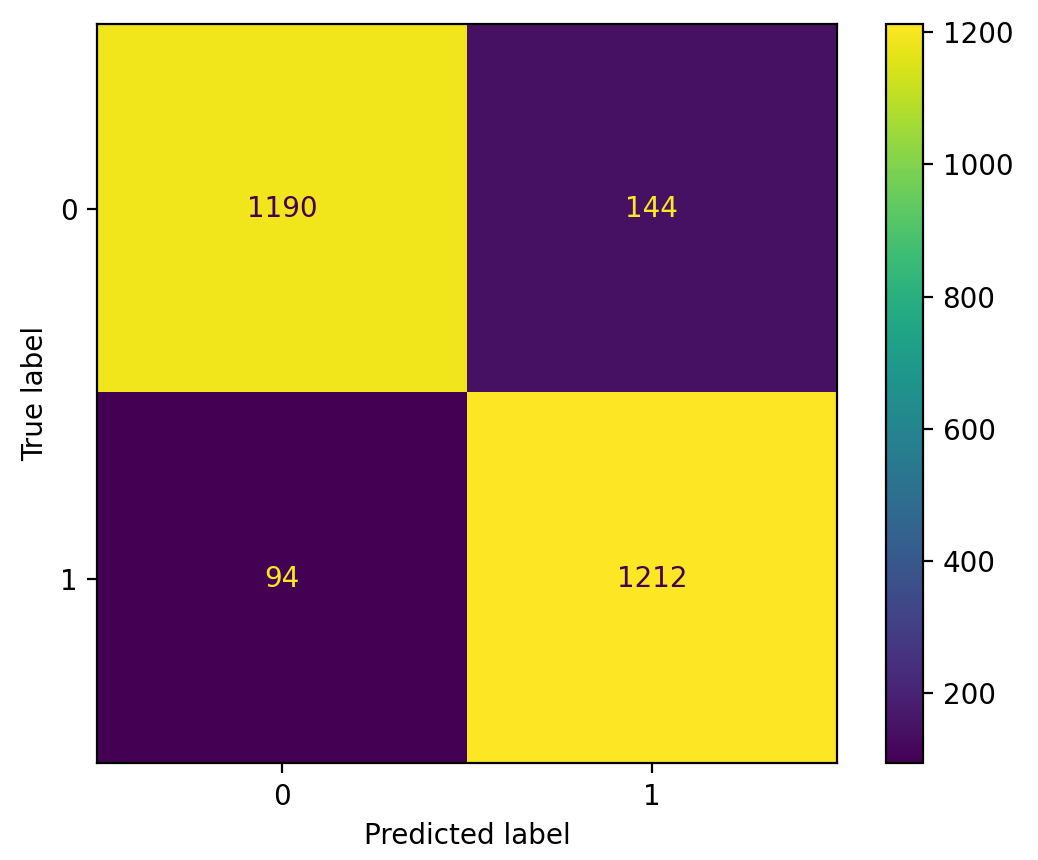
\includegraphics[width=.5\textwidth]{images/confusion_matrix_GDA.png}
    \caption{GDA模型的混淆矩阵}
    \label{fig:confusion-matrix-GDA}
\end{figure}
在数据分布不平衡的情况下,GDA对于破产标签的召回率为0.21,也即找出了20\%的破产
公司,模型准确率40.7\%,F1值为0.28。

\paragraph{随机森林}
\textit{PCA}中选择27个主成分,随机森林中决策树数量选择100棵,
采用\textit{Bootstrap}方法生成每颗树的训练样本,迭代训练直到
收敛。在原始的测试集上进行测试,得到的混淆矩阵展示在图\ref{fig:confusion-matrix-random-forest}中。
\begin{figure}[ht]
    \centering
    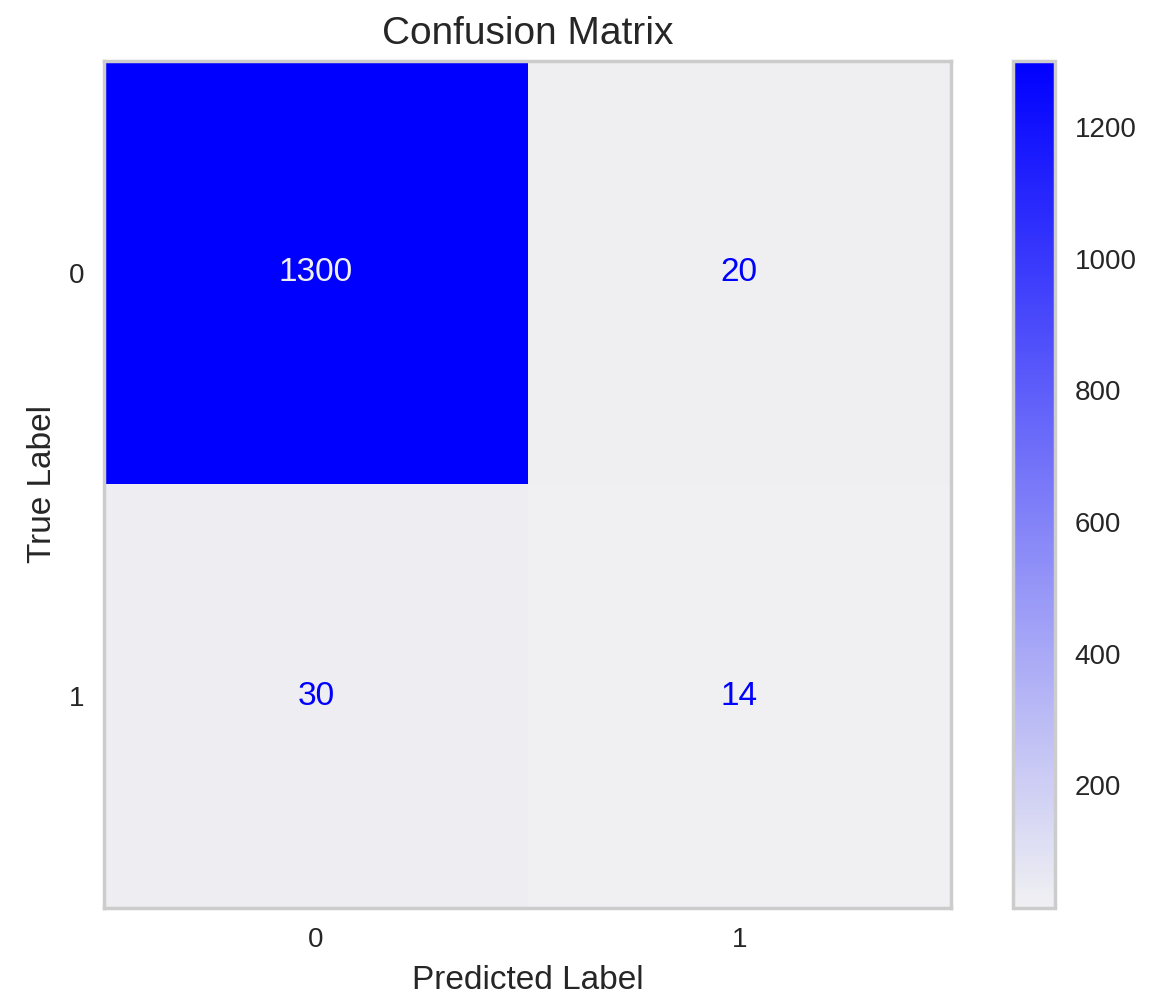
\includegraphics[width=.5\textwidth]{images/random_forest_confusion_matrix_unbalanced.png}
    \caption{随机森林模型的混淆矩阵}
    \label{fig:confusion-matrix-random-forest}
\end{figure}
随机森林模型准确率41.2\%,F1值为0.36。